\documentclass{beamer}

\usepackage[utf8]{inputenc}
\usepackage[russian]{babel}

\usepackage{graphicx}
\usepackage{gensymb}

\usefonttheme[onlymath]{serif}

%\usepackage{beamerthemesplit}
%\useoutertheme{infolines}
%\useoutertheme{smoothtree}
\useoutertheme{tree}
\useinnertheme{circles}
\setbeamertemplate{itemize items}[default]
\setbeamertemplate{enumerate items}[default]

\definecolor{myblue}{rgb}{.0,.2,.3}
\setbeamercolor*{palette primary}{use=structure,fg=white,bg=myblue}
\setbeamertemplate{navigation symbols}{}

\usepackage{tikz}
\usetikzlibrary{shapes.geometric, arrows, trees}
\tikzstyle{every node}=[font=\tiny, node distance=0.8cm]
\tikzstyle{io} = [trapezium, trapezium left angle=70, trapezium right angle=110, minimum width=1cm, minimum height=0.33cm, text centered, text width=1cm, draw=black, fill=blue!30]
\tikzstyle{process} = [rectangle, minimum width=1cm, minimum height=0.31cm, text centered, draw=black, fill=orange!30]
\tikzstyle{decision} = [diamond, minimum width=1cm, minimum height=0.31cm, text centered, draw=black, fill=green!30]
\tikzstyle{arrow} = [thick,->,>=stealth]
\tikzstyle{bigrect} = [rectangle, minimum width=5.5cm, minimum height=4.5cm, text depth=5cm, draw=black, dashed]

%\usepackage{verbatim}
\usepackage{listings}
%\usepackage{enumitem}
%\setlistdepth{9}
%\setlist[itemize,1]{label=$\bullet$}
%\setlist[itemize,2]{label=$\bullet$}
%\setlist[itemize,3]{label=$\bullet$}
%\setlist[itemize,4]{label=$\bullet$}
%\setlist[itemize,5]{label=$\bullet$}
%\setlist[itemize,6]{label=$\bullet$}
%\setlist[itemize,7]{label=$\bullet$}
%\setlist[itemize,8]{label=$\bullet$}
%\setlist[itemize,9]{label=$\bullet$}
%\renewlist{itemize}{itemize}{9}

\newcommand{\layersInRealLife} {
  \frametitle{Уровни (levels / layers) в реальной жизни}
  \framesubtitle{Уровни характеризуются \textbf{обязанностями} и определяют \textbf{кто над кем главнее (выше)}}

  \begin{itemize}
    \item Директор конторы (высокий уровень)
      \begin{itemize}
        \item Художник (низкий уровень)
        \item Программист (низкий уровень)
        \begin{itemize}
          \item Младший программист (самый низкий уровень)
        \end{itemize}
      \end{itemize}
  \end{itemize}
}

\newcommand{\paradigmsImpDecl} {
  \node (imper) [bigrect, xshift=-1cm] {Императивное};
  \node (decl) [bigrect, xshift=5cm, yshift=2.5cm] {Декларативное};
}

\newcommand{\paradigmsAlg} {
  \paradigmsImpDecl

  \node (alg) [process, dashed, xshift=-1cm, yshift=1cm] {Алгоритмическое};
    \node [xshift=-1cm, yshift=0.65cm] {Блок-схемы, словесное описание};
}

\newcommand{\paradigmsStruct} {
  \paradigmsAlg

  \node (struct) [process, xshift=0cm, yshift=0cm] {Структурное};
    \node [xshift=0cm, yshift=-0.35cm] {Ограничение алгоритмического};
  \draw [arrow] (alg) -- (struct);
}

\newcommand{\paradigmsProc} {
  \paradigmsStruct

  \node (proc) [process, xshift=-1cm, yshift=-1cm] {Процедурное};
    \node [xshift=-1cm, yshift=-1.35cm] {C, Pascal...};
  \draw [arrow] (struct) -- (proc);
}

\newcommand{\paradigmsOop} {
  \paradigmsProc

  \node (oop) [process, xshift=-1.5cm, yshift=-2cm] {Объектно-ориентированное (ООП)};
    \node [xshift=-1.5cm, yshift=-2.35cm] {C++, C\#, Java, Python, Ruby, JS, ...};
  \draw [arrow] (proc) -- (oop);
}

\newcommand{\paradigmsDecls} {
  \paradigmsOop

  \node (notprog) [process, dashed, xshift=5cm, yshift=4cm] {Описания};
    \node [xshift=5cm, yshift=3.65cm] {Конфигурации и Web API (XML, JSON),};
    \node [xshift=5cm, yshift=3.35cm] {вёрстка (HTML, LaTeX), аннотации};
}

\newcommand{\paradigmsFunc} {
  \paradigmsDecls

  \node (func) [process, xshift=4cm, yshift=2.5cm] {Функциональное};
}

\newcommand{\paradigmsLogical} {
  \paradigmsFunc

  \node (logical) [process, xshift=5cm, yshift=1cm] {Логическое};
}

\newcommand{\paradigmsAll} {
  \paradigmsLogical

  \node (generic) [process, xshift=-1cm, yshift=5cm] {Обобщенное};
  \node (concurrent) [process, xshift=5cm, yshift=-2cm] {Конкурентное};
  \node (module) [process, xshift=-2cm, yshift=4cm] {Модульное};
}


\title{Введение в программирование}
\author{Лопатин Александр}
\date{2015}


\subtitle{Лекция 1}

\begin{document}

  \frame{\titlepage}


  \section*{Содержание} {
    \frame{\tableofcontents[hideallsubsections]}


  \section{О чем курс}
    \frame {
      \begin{itemize}
        \item урезанная версия одноименного универовского курса (обычно рассчитанного на 1---2 семестра)
        \item основы и упоминания из других курсов
      \end{itemize}
    }

    \frame {
      \frametitle{Expectations}
      \begin{itemize}
        \item получим кругозор
        \item узнаем основы нескольких языков
        \item научимся базовым техникам
        \item на практике применим некоторые техники
      \end{itemize}
    }


  \section{Как построен курс}
    \frame {
      \begin{itemize}
        \item разбит так, чтобы не вызвать передоз информацией
        \item одно занятие в неделю на 2---3 часа (включает лекцию и практику)
        \item 10 недель ($\approx 2\frac{1}{3}$ месяца)
        \item домашки на не более 2-х часов в неделю
        \item один мелкий проект на 2 недели (2 викенда)
        \item домашки и проект будут оцениваться
      \end{itemize}
    }


  \section{Вводные термины}
    \frame {
      \frametitle{Исполнитель}
      \begin{itemize}
        \item повар
        \item военнослужащий
        \item гитарист
        \item рок-группа
        \item коммерческая компания
        \item вычислительная система (компьютер, смартфон, бытовой прибор и т.п.)
      \end{itemize}
    }

    \frame {
      \frametitle{Инструкции исполнителя}
      \begin{itemize}
        \item \textbf{пункты рецепта} (<<42. Положить ложку сахара>>) для повара
        \item \textbf{приказы} (<<нале-во!>>) для военнослужащего
        \item \textbf{аккорды} для гитариста 
        \item \textbf{инструкции процессора} (<<сложить два числа>>) для вычислительной системы
      \end{itemize}
    }

    \frame {
      \frametitle{Алгоритм}
      Конечная последовательность \textbf{инструкций исполнителя} направленная на решение задачи
      \vspace{1cm}
      \begin{itemize}
        \item \textbf{рецепт} для повара
        \item \textbf{лабораторная работа} для студента
        \item \textbf{текст песни} для вокалиста
        \item \textbf{бизнес-план} коммерческой компании
        \item \textbf{шаги воспроизведения проблемы} для тестировщика
        \item \textbf{компьютерная программа} для вычислительной системы
      \end{itemize}
    }

    \frame {
      \frametitle{Интерфейс}
        Взаимодействие
        \vspace{0.5cm}
        \begin{itemize}
          \item Пользовательский (UI --- User Interface)
            \begin{itemize}
              \item Графический пользовательский интерфейс, Graphical User Interface (GUI)
              \item Интерфейс коммандной строчки, Command-Line Interface (CLI)
            \end{itemize}
          \item Программный (API --- Application Interface)
            \begin{itemize}
              \item подпрограммы, модули, библиотеки
              \item сетевые протоколы (например HTTP)
              \item много других
            \end{itemize}
        \end{itemize}
        \vspace{0.5cm}
        CLI может использоваться как API
    }

  \section{Обзор развития вычислительных систем}
    \frame {
      \frametitle{1945: Архитектура фон Неймана (Von Neumann architecture)}
      \begin{center}
        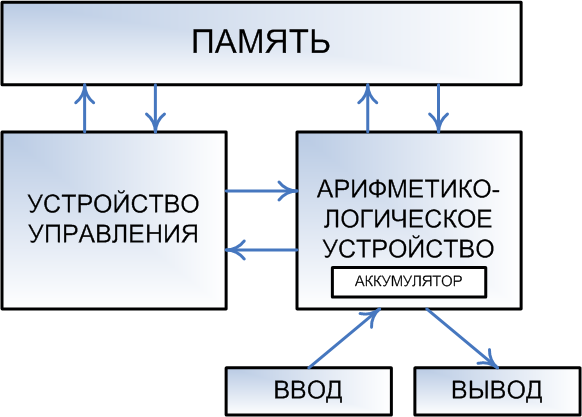
\includegraphics[scale=1]{pictures/Von_Neumann_architecture.png}
      \end{center}
    }

    \frame {
      \frametitle{1946: ENIAC}
      \begin{center}
        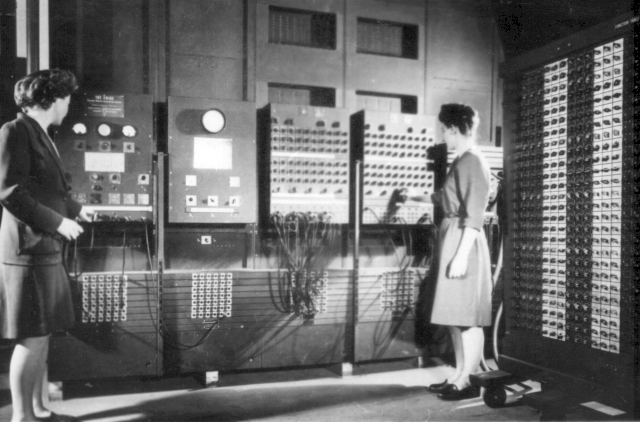
\includegraphics[scale=0.4]{pictures/ENIAC.png}
      \end{center}
    }

    \frame {
      \frametitle{1964: IBM System/360}
      \begin{center}
        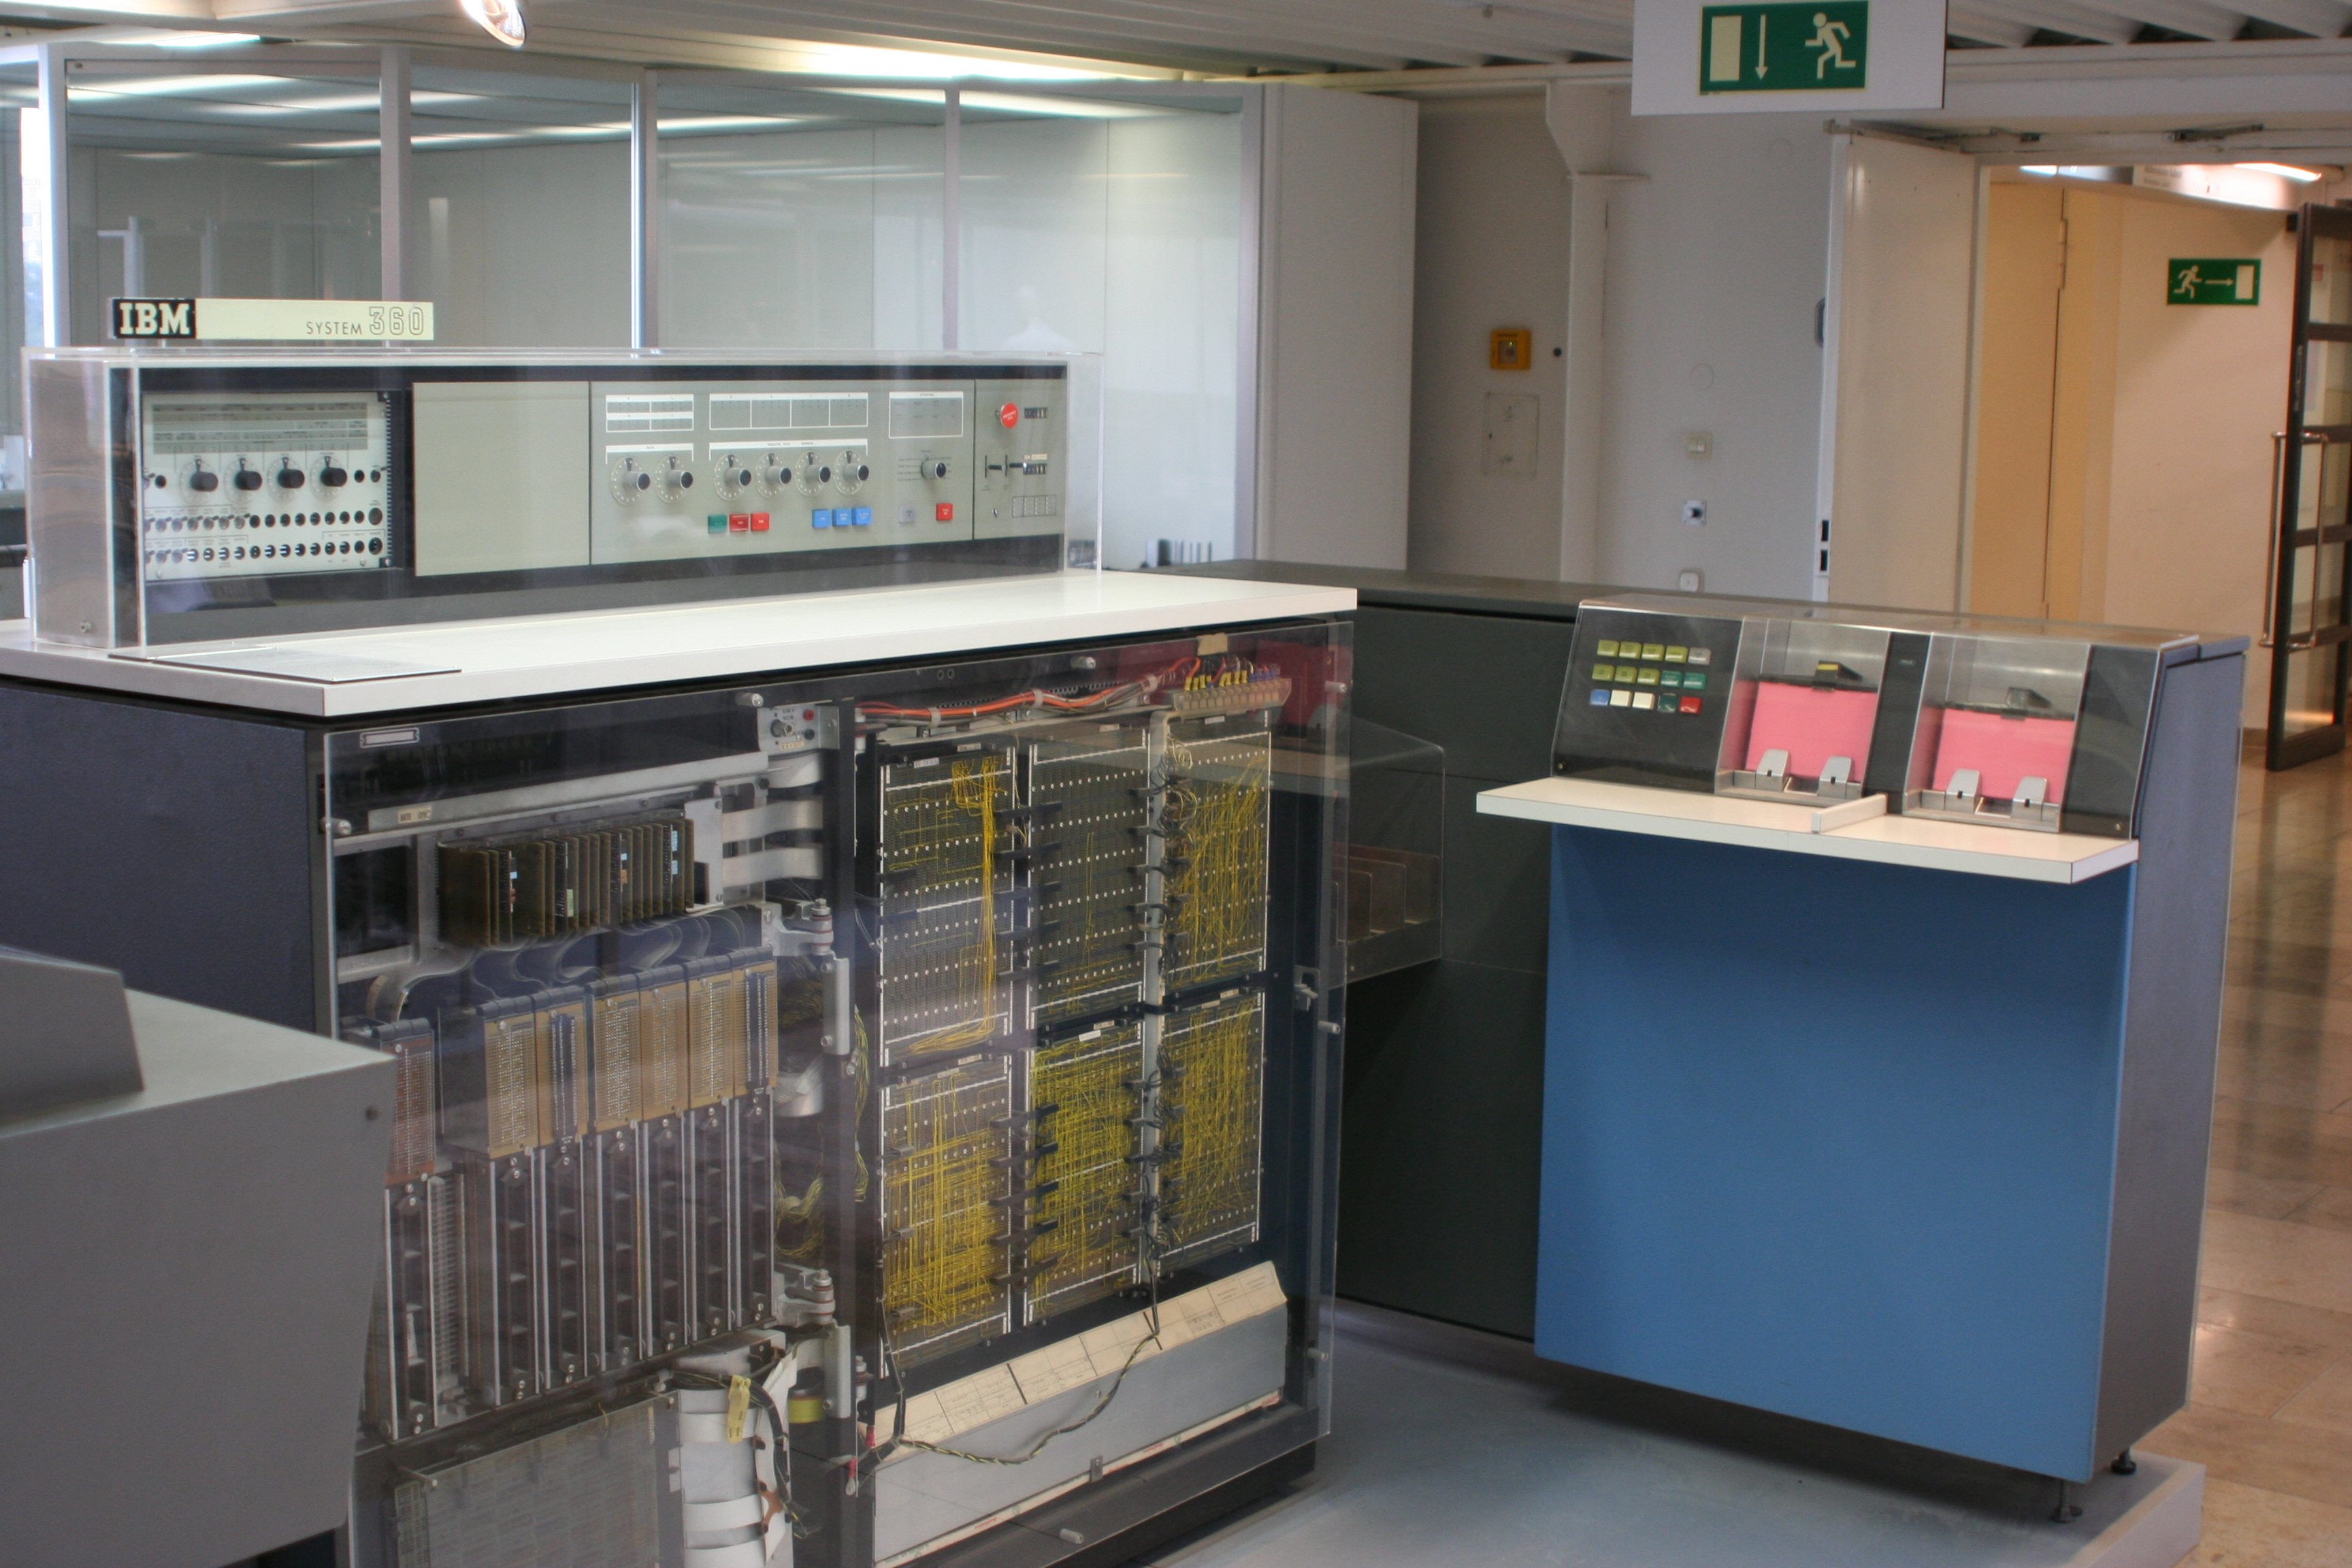
\includegraphics[scale=0.07]{pictures/IBM_S360.jpg}
      \end{center}
    }

%    \frame {
%      \frametitle{<<Хакерская этика>> 60-ых}
%      В 60-е значение слова <<Хакер>> еще не было испорчено журналистами
%      \begin{itemize}
%        \item Доступ к компьютерам и любым другим средствам познания устройства мира для каждого должен быть неограниченным
%        \item Информация должна быть свободной
%        \item Недоверие властям и продвижение принципа децентрализации
%        \item Оценивать хакера можно лишь по его достижениям. Ни положение в обществе, ни возраст, ни раса не играют при этом никакой роли
%      \end{itemize}
%
%      \vspace{0.5cm}
%      
\includegraphics[scale=0.05]{../../common/book.png}~Стивен Леви --- Хакеры: Герои компьютерной революции
%    }

    \frame {
      \frametitle{1975: Закон Мура}
      \begin{center}
        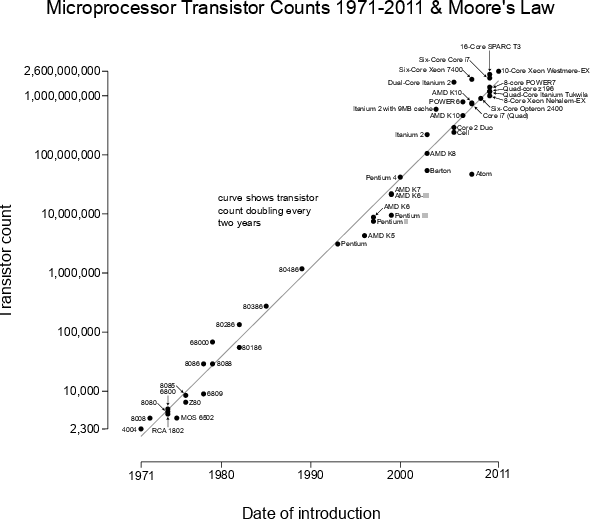
\includegraphics[scale=0.4]{pictures/moore_law.png}
      \end{center}
    }

    \frame {
      Закон прекратил действовать --- пришло время новых идей по увеличению производительности железа

      \vspace{0.5cm}
      \begin{itemize}
        \item выполнять трудоемкие операции на других устройствах (например GPU)
        \item объединять несколько ядер процессоров в один
        \item объединять несколько компьютеров в вычислительный кластер
        \item проектировать концептуально другие выч. системы, необязательно на основе фон Неймовской архитектуры
        \begin{itemize}
          \item квантовые компьютеры
          \item клеточные компьютеры
          \item ...
        \end{itemize}
      \end{itemize}
    }

    \frame {
      С ростом производительности железа растет и сложность задач

      \vspace{0.5cm}
      Сложность программ тоже растет

      \vspace{0.5cm}
      Появляется много специализаций в IT, по аналогии с врачами
    }

    \frame {
      \frametitle{Многоуровневые системы}
      Системы состоят из подсистем (из слоёв / уровней)
      \begin{center}
        
\includegraphics[scale=0.4]{../../common/you_dont_say.png}
      \end{center}
    }

    \frame {
      \layersInRealLife
    }

    \frame {
      \frametitle{Каждая железяка состоит из множества поджелезяк}
      \begin{center}
        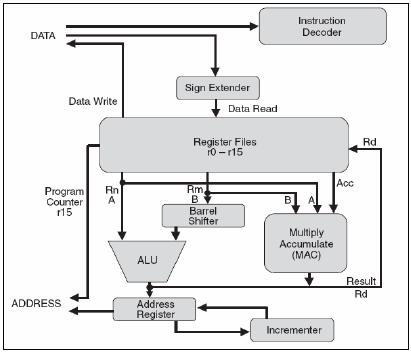
\includegraphics[scale=0.7]{pictures/arm-arch.png}
      \end{center}
    }

    \frame {
      \frametitle{Софт тоже многоуровневый}

      \begin{center}
        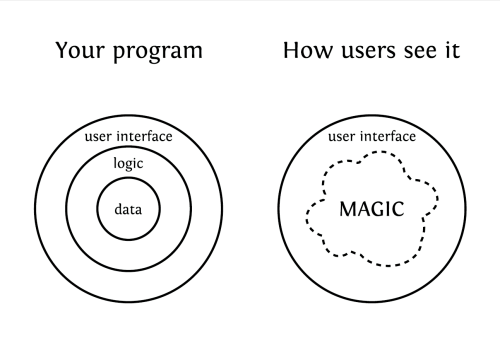
\includegraphics[scale=0.7]{pictures/programs-as-seen-by-users.png}
      \end{center}
    }

  \section{Парадигмы программирования}
    \frame {
      \begin{tikzpicture}
        \node (imper) [bigrect, xshift=-1cm] {Императивное};
          \node (alg) [process, dashed, xshift=-1cm, yshift=1cm] {Алгоритмическое};
            \node [xshift=-1cm, yshift=0.65cm] {Блок-схемы, словесное описание};
          \node (struct) [process, xshift=0cm, yshift=0cm] {Структурное};
            %\node [xshift=0cm, yshift=-0.35cm] {Fortran...};
          \node (proc) [process, xshift=-1cm, yshift=-1cm] {Процедурное};
            \node [xshift=-1cm, yshift=-1.35cm] {C, Pascal...};
          \node (oop) [process, xshift=-1.5cm, yshift=-2cm] {Объектно-ориентированное (ООП)};
            \node [xshift=-1.5cm, yshift=-2.35cm] {C++, C\#, Java, Python, Ruby, JS, ...};

        \node (decl) [bigrect, xshift=5cm] {Декларативное};

        \draw [arrow] (alg) -- (struct);
        \draw [arrow] (struct) -- (proc);
        \draw [arrow] (proc) -- (oop);
      \end{tikzpicture}
    }

    \frame {
      \frametitle{Императивное программирование (Imperative Programming)}

      Написание \textbf{алгоритмов} путём перечисления \textbf{инструкций исполнителя}
      \vspace{0.5cm}
      \begin{center}
        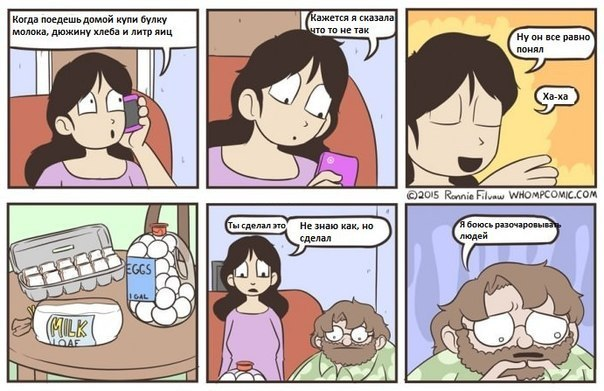
\includegraphics[scale=0.5]{pictures/imperative-programmer.jpg}
      \end{center}
    }

    \begin{frame}
      \frametitle{Декларативное программирование (Declarative Programming)}
      \textbf{Описание желаемого результата}, \underline{вместо алгоритма} получения этого результата.\linebreak
        \vspace{0.5cm}

        Например запрос к базе данных:

        \vspace{0.5cm}
        \texttt{Выбрать абитуриентов}

        \texttt{поступающих на специальность <<Программная Инженерия>>}

        \texttt{с сортировкой по сумме баллов по убыванию}
        \vspace{1cm}

        Подробнее рассмотрим ближе к концу курса
    \end{frame}


  \section{Алгоритмическое программирование}

    \subsection{Словесное описание}
      \frame {
        \frametitle{Линейный алгоритм}
        \begin{enumerate}
          \item Шагнуть вперед
          \item Шагнуть вперед
          \item Повернуть направо на $90^\circ$
          \item Шагнуть вперед
        \end{enumerate}
      }

      \frame {
        \frametitle{Алгоритм с ветвлением}

        \vspace{0.5cm}
        1. Для каждого студента
        \begin{itemize}
          \item 1.1. Напечатать имя, фамилию
          \item 1.2. Если балл <= 2 перейти к п. 1.2.1 иначе к п. 1.3
          \begin{itemize}
            \item 1.2.1. Задать красный цвет шрифта
          \end{itemize}
          \item 1.3. Напечатать оценку
          \item 1.4. Задать черный цвет шрифта
        \end{itemize}
      }

    \subsection{Язык блок-схем}
      \frame {
        \frametitle{Линейный алгоритм}
      }

      \frame {
        \frametitle{Алгоритм с ветвлением}
      }

%      \frame {
%        \begin{tikzpicture}
%          \node (in1) [io] {Input};
%          \node (pro1) [process, below of=in1] {Process 1};
%          \node (dec1) [decision, below of=pro1, yshift=-0.5cm] {Decision 1};
%          \node (pro2a) [process, below of=dec1, yshift=-0.5cm] {Process 2a};
%          \node (pro2b) [process, right of=dec1, xshift=2cm] {Process 2b};
%          \node (out1) [io, below of=pro2a] {Output};
%          \draw [arrow] (pro2b) |- (pro1);
%          \draw [arrow] (pro2a) -- (out1);
%        \end{tikzpicture}
%      }

      \frame {
        \frametitle{Практика}
      }


  \section{Структурное программирование}
    \frame {
      \frametitle{Structured Programming}
      \begin{itemize}
        \item отказ от безусловного перехода
        \item использование двух \textbf{управляющих структур}
        \begin{itemize}
          \item условие
          \item цикл
        \end{itemize}
      \end{itemize}
    }

    \frame {
      \frametitle{Цикл с предусловием}
    }

    \frame {
      \frametitle{Цикл со счетчиком --- частный случай цикла с предусловием}
    }

    \frame {
      \frametitle{Цикл с постусловием}
    }

    \frame {
      \frametitle{Пример алгоритма}
    }

    \frame {
      \frametitle{Практика}
    }


\end{document}

% vim:shiftwidth=2:softtabstop=2:tabstop=2
